\documentclass[main.tex]{subfiles}
\begin{document}
\chapter{Integration framework}
\thispagestyle{chapstyle}
\label{chap_framework}
\minitoc

In this chapter, we propose a framework enabling the integration of multiple applications on the \mppalong following the execution model defined in Chapter~\ref{chap_execModel} and thus, in a time-composable manner. Overall, the whole framework relies on the property of \emph{temporal isolation} that is provided to partitions. As shown in Figure~\ref{fig_framework_workFlow}, we propose to integrate partitions using a \emph{work-flow} going from the applications' models down to an executable that runs on the target in a predictable manner. In this work-flow, several off-line computations need to be achieved in order to build scheduling tables that will be enforced at run-time on the \mppalong with a hypervisor. 
We will firstly present what the inputs of this work-flow are and we will explain and formalize the notion of \emph{resource budget} of a partition. Then, we will overview the two different operations that are computed off-line based on the models of partitions. Finally, we will detail the purpose of having on-line support for the partitions using a hypervisor. 

\begin{figure}
    \centering
    \scalebox{0.9}{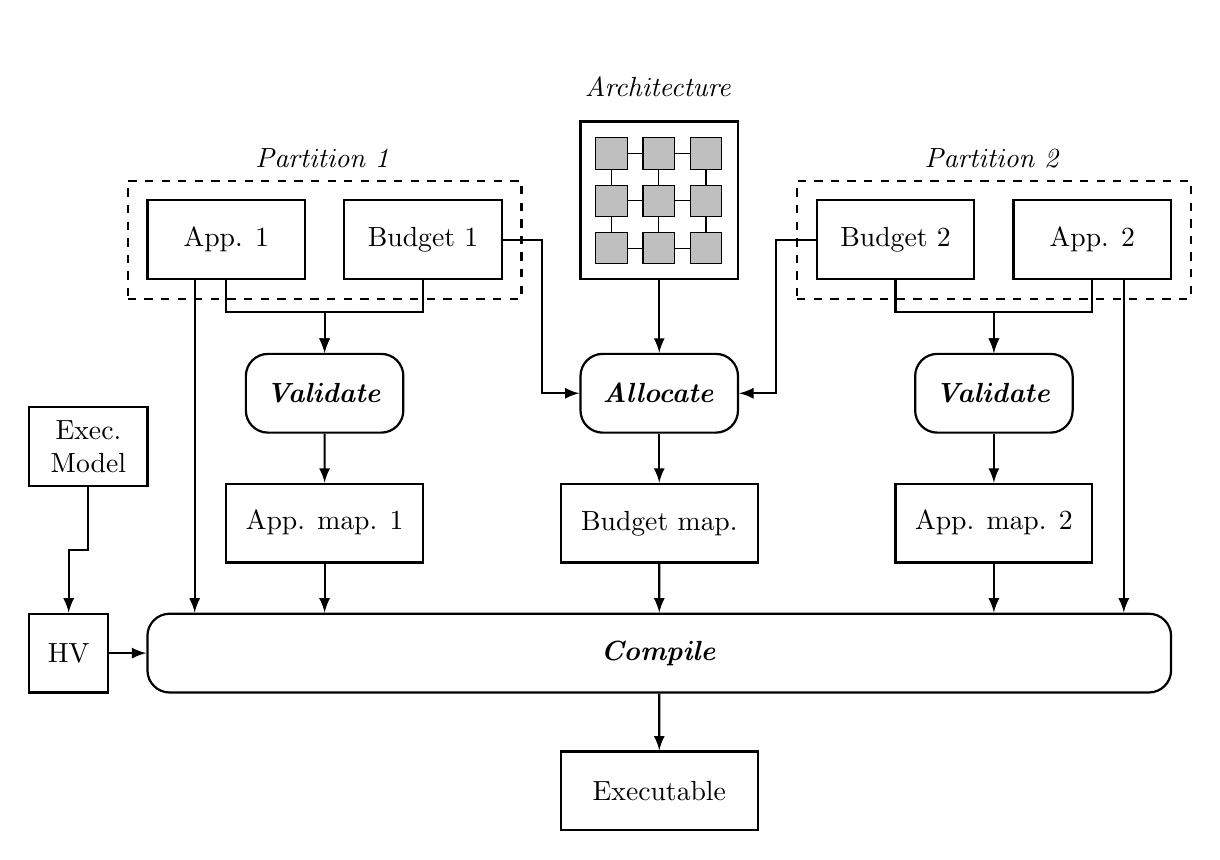
\begin{tikzpicture}
\draw (5.5,0) node[draw, rectangle, inner sep=0pt, minimum width=2cm, minimum height=2cm, anchor=south west, thick] (Archi) {};
\draw (5.7,0.2) node[draw, rectangle, inner sep=0pt, minimum width=0.4cm, minimum height=0.4cm, anchor=south west, fill=lightgray] (t11) {};
\draw (6.3,0.2) node[draw, rectangle, inner sep=0pt, minimum width=0.4cm, minimum height=0.4cm, anchor=south west, fill=lightgray] (t12) {};
\draw (6.9,0.2) node[draw, rectangle, inner sep=0pt, minimum width=0.4cm, minimum height=0.4cm, anchor=south west, fill=lightgray] (t13) {};
\draw (5.7,0.8) node[draw, rectangle, inner sep=0pt, minimum width=0.4cm, minimum height=0.4cm, anchor=south west, fill=lightgray] (t21) {};
\draw (6.3,0.8) node[draw, rectangle, inner sep=0pt, minimum width=0.4cm, minimum height=0.4cm, anchor=south west, fill=lightgray] (t22) {};
\draw (6.9,0.8) node[draw, rectangle, inner sep=0pt, minimum width=0.4cm, minimum height=0.4cm, anchor=south west, fill=lightgray] (t23) {};
\draw (5.7,1.4) node[draw, rectangle, inner sep=0pt, minimum width=0.4cm, minimum height=0.4cm, anchor=south west, fill=lightgray] (t31) {};
\draw (6.3,1.4) node[draw, rectangle, inner sep=0pt, minimum width=0.4cm, minimum height=0.4cm, anchor=south west, fill=lightgray] (t32) {};
\draw (6.9,1.4) node[draw, rectangle, inner sep=0pt, minimum width=0.4cm, minimum height=0.4cm, anchor=south west, fill=lightgray] (t33) {};
\draw (t11) -- (t12) -- (t13); 
\draw (t21) -- (t22) -- (t23); 
\draw (t31) -- (t32) -- (t33); 
\draw (t11) -- (t21) -- (t31); 
\draw (t12) -- (t22) -- (t32); 
\draw (t13) -- (t23) -- (t33); 

\draw (5.5,1.7) node[inner sep=0pt, minimum width=2cm, minimum height=1.5cm, anchor=south west] {\textit{Architecture}};

\draw (0,0) node[draw, rectangle, inner sep=0pt, minimum width=2cm, minimum height=1cm, anchor=south west, thick] (App1) {App. 1};
\draw (2.5,0) node[draw, rectangle, inner sep=0pt, minimum width=2cm, minimum height=1cm, anchor=south west, thick] (Bud1) {Budget 1};
\draw (8.5,0) node[draw, rectangle, inner sep=0pt, minimum width=2cm, minimum height=1cm, anchor=south west, thick] (Bud2) {Budget 2};
\draw (11,0) node[draw, rectangle, inner sep=0pt, minimum width=2cm, minimum height=1cm, anchor=south west, thick] (App2) {App. 2};

\draw (-0.25,-0.25) node[draw, rectangle, inner sep=0pt, minimum width=5cm, minimum height=1.5cm, anchor=south west, thick, dashed] {};
\draw (-0.25,0.8) node[inner sep=0pt, minimum width=5cm, minimum height=1.5cm, anchor=south west] {\textit{Partition 1}};
\draw (8.25,-0.25) node[draw, rectangle, inner sep=0pt, minimum width=5cm, minimum height=1.5cm, anchor=south west, thick, dashed] {};
\draw (8.25,0.8) node[inner sep=0pt, minimum width=5cm, minimum height=1.5cm, anchor=south west] {\textit{Partition 2}};

\draw (5.5,-1.95) node[draw, rectangle, inner sep=0pt, minimum width=2cm, minimum height=1cm, anchor=south west, rounded corners=8pt, thick] (Alloc) { \textbf{\textit{Allocate}}};
\draw (1.25,-1.95) node[draw, rectangle, inner sep=0pt, minimum width=2cm, minimum height=1cm, anchor=south west, rounded corners=8pt, thick] (Valid1) {\textbf{\textit{Validate}}};
\draw (9.75,-1.95) node[draw, rectangle, inner sep=0pt, minimum width=2cm, minimum height=1cm, anchor=south west, rounded corners=8pt, thick] (Valid2) {\textbf{\textit{Validate}}};

\draw[-latex, thick] (App1.south) -- ([yshift=-4mm]App1.south) -| (Valid1.north);
\draw[-latex, thick] (Bud1.south) -- ([yshift=-4mm]Bud1.south) -| (Valid1.north);
\draw[-latex, thick] (App2.south) -- ([yshift=-4mm]App2.south) -| (Valid2.north);
\draw[-latex, thick] (Bud2.south) -- ([yshift=-4mm]Bud2.south) -| (Valid2.north);
\draw[-latex, thick] (Bud1.east) -- ([xshift=5mm]Bud1.east) |- (Alloc.west);
\draw[-latex, thick] (Bud2.west) -- ([xshift=-5mm]Bud2.west) |- (Alloc.east);
\draw[-latex, thick] (Archi.south) --  (Alloc.north);

\draw (1,-3.6) node[draw, rectangle, inner sep=0pt, minimum width=2.5cm, minimum height=1cm, anchor=south west, thick] (AppMap1) {App. map. 1};
\draw (5.25,-3.6) node[draw, rectangle, inner sep=0pt, minimum width=2.5cm, minimum height=1cm, anchor=south west, thick] (BudMap) {Budget map.};
\draw (9.5,-3.6) node[draw, rectangle, inner sep=0pt, minimum width=2.5cm, minimum height=1cm, anchor=south west, thick] (AppMap2) {App. map. 2};

\draw[-latex, thick] (Valid1.south) --  (AppMap1.north);
\draw[-latex, thick] (Valid2.south) --  (AppMap2.north);
\draw[-latex, thick] (Alloc.south) --  (BudMap.north);    

\draw (-1.5,-2.625) node[draw, rectangle, inner sep=0pt, minimum width=1.5cm, minimum height=1cm, anchor=south west, text width=1.25cm, align=center, thick] (EM) {Exec. \\ Model};

\draw (-1.5,-5.25) node[draw, rectangle, inner sep=0pt, minimum width=1cm, minimum height=1cm, anchor=south west, thick] (HV) {HV};

\draw[-latex, thick] (EM.south) -- ([yshift=-8mm]EM.south) -| (HV.north);

\draw (0,-5.25) node[draw, rectangle, inner sep=0pt, minimum width=13cm, minimum height=1cm, anchor=south west, rounded corners=8pt, thick] (Compile) {\textbf{\textit{Compile}}};

\draw[-latex, thick] (AppMap1.south) --  (AppMap1|-Compile.north);
\draw[-latex, thick] (AppMap2.south) --  (AppMap2|-Compile.north);
\draw[-latex, thick] (BudMap.south) --  (Compile.north);
\draw[-latex, thick] ([xshift=-4mm]App1.south) --  ([xshift=-4mm]App1.south|-Compile.north);
\draw[-latex, thick] ([xshift=4mm]App2.south) --  ([xshift=4mm]App2.south|-Compile.north);
\draw[-latex, thick] (HV.east) --  (Compile.west);

\draw (5.25,-7) node[draw, rectangle, inner sep=0pt, minimum width=2.5cm, minimum height=1cm, anchor=south west, thick] (exec) {Executable};
\draw[-latex, thick] (Compile.south) --  (exec.north);


\end{tikzpicture}

}
    \caption{Integration of partitions on the \mppalong work-flow}
    \label{fig_framework_workFlow}
\end{figure}


\section{Input parameters}
The purpose of the work-flow shown in Figure~\ref{fig_framework_workFlow} is to integrate temporally isolated partitions on the \mppalong. The inputs of this workflow include a model of the hardware platform and a set of partitions. Each partition is composed of an application and a \emph{resource budget}. We detail how these inputs are structured below. 


\subsection{Platform model}
\label{ssec_framework_hwModel}
The hardware target that is considered in this thesis is the \mppalong. We already detailed its architecture in Section~\ref{sec_systemModel_archiMppa} and provided models of its shared resources in Section~\ref{sec_execModel_boundsSharedRes}. For convenience, we formalize the \mppalong as a tuple 
$< C_K , I_K , N_K, R_K >$ where:
\begin{itemize}
    \item $C_K = \{ c_K^0 , \ldots , c_K^{15} \}$ represent the 16 compute clusters.
    \item $I_K = \{ i_K^0 , \ldots , i_K^{15} \}$ represent the 16 I/O RMs.
    \item $N_K = \{ n_K^0 , \ldots , n_K^{31} \}$ represent the 32 NoC nodes.
    \item $R_K = \bigcup R_K^{ij}$ is the set of all NoC routes with $R_K^{ij}$ the set of routes connecting the NoC node $n_K^i$ to the NoC node $n_K^j$.
\end{itemize}


\subsection{Resource budget}
\label{ssec_framework_partitionModel}
As shown in Figure~\ref{fig_framework_workFlow}, a partition consists of an application provided together with a \emph{resource budget}. We assume the applications to fit in the model of Section~\ref{sec_systemModel_appModel}. A resource budget consists of the amount of resources required by an application to be executed. More formally, the resource budget of a partition $P_i$ is defined as a tuple $<\mathcal{N}_i, \mathcal{I}_i, \mathcal{C}_i, \mathcal{B}_i>$ where:
    \begin{enumerate}
        \item $\mathcal{N}_i = \{ pn_1^i , \ldots , pn_n^i \}$ is a finite set of \emph{Partition Nodes} (or \emph{\PN{}s}). A \PN{} represents a need in computational power for a partition inside a compute cluster. Each \PN{} is associated with a number of PEs and a number of local SRAM banks. More formally: 
            \begin{itemize}
                \item $N_c : \mathcal{N}_i \mapsto \mathbb{N}$ associates each \PN{} with the number of PEs that needs to be reserved for it in a compute cluster.
                \item $N_b : \mathcal{N}_i \mapsto \mathbb{N}$ associates each \PN{} with the number of local SRAM banks that need to be allocated to it in a compute cluster.
            \end{itemize}

        \item  $\mathcal{I}_i = \{ io_1^i , \ldots , io_o^i \}$ is a finite set of \emph{I/O Nodes} (or \emph{\ION{}s}). An \ION{} is an access point to the external DDR-SDRAM. It is materialized by a RM core located on an I/O cluster. It answers remote reads and remote writes requests between \PN{}s and external memory banks.
    
        \item $\mathcal{C}_i = \{ pc_1^i , \ldots , pc_p^i \}$ is a finite set of \emph{Partition Communications} (or \emph{\PC{}s}). A \PC{} is a directed communication channel for \PN{}s placed on different compute clusters (or between a \PN{} and an \ION{}). It is materialized as a strictly periodic access to the NoC for sending message from a \PN{}/\ION{} to a remote \PN{}/\ION{}. More formally:
            \begin{itemize}
                \item $src : \mathcal{C}_i \mapsto \mathcal{N}_i \cup \mathcal{I}_i$ associates each \PC{} with its source \PN{} or \ION{}.
                \item $dst : \mathcal{C}_i \mapsto \mathcal{N}_i \cup \mathcal{I}_i$ associates each \PC{} with its destination \PN{} or \ION{}.
                \item $T : \mathcal{C}_i \mapsto \mathbb{N}$ provides the \emph{period} of activation of the \PC{}.
                \item $C : \mathcal{C}_i \mapsto \mathbb{N}$ provides the \emph{duration} of the \PC{}'s NoC access slot.
                \item $O : \mathcal{C}_i \mapsto \mathbb{N}$ provides the \emph{offset} of the \PC{}, also denoted as the first activation date.
                \item $R : \mathcal{C}_i \mapsto \mathbb{N}$ provides the maximum number of NoC nodes of the route taken by the \PC{}. It can be used to impose a constraint of maximal latency.

            \end{itemize}

        \item $\mathcal{B}$ represents a number of external DDR-SDRAM banks.
    \end{enumerate}

    All together, a partition includes the actual application and a set of \emph{abstract} resources formalized under the notion of \emph{budget}. Doing so enables application designers to express their needs for hardware resources and to request them early in the development process. This sort of resource reservation policy helps design, develop, test and qualify applications without having the knowledge of co-running partitions. Once a partition has its boundaries defined formally, the utilization of all other resources on the target becomes of little interest since it cannot have an impact on the application running inside the partition thanks to our execution model. Yet, the execution model requires both off-line and on-line support to be enforced. We detail how this is implemented respectively in sections~\ref{sec_framework_offLineComputations} and~\ref{sec_framework_onLineSupport}.


\section{Off-line computations}
\label{sec_framework_offLineComputations}
As shown in Figure~\ref{fig_framework_workFlow}, our work-flow includes two different off-line phases. During the \emph{Validate} phase, the models of applications are checked over their allocated budgets. By doing so, we verify if the resources allocated to a partition are sufficient to execute the application and to meet all its constraints (both functional and non-functional). During the \emph{Allocate} phase, the abstract resources of the budgets are matched over concrete resources on the hardware platform. In other words, the \emph{Allocate} phase assigns \PN{}s to clusters, \PC{}s to NoC routes and \ION{}s to RMs on I/O clusters in such a way that partitions do not overlap. Both the \emph{Validate} and \emph{Allocate} phases are currently implemented using Constraint Programming and are fully automated. We detail the operations achieved during these two phases below.

\subsection{Validate}
During the \emph{Validate} phase, applications are checked over their budgets. Using the application model defined in Section~\ref{sec_systemModel_appModel}, a budget will essentially be considered as valid if a schedule of all sub-tasks on \PN{}s and a mapping of data on \PC{}s can be found. More precisely, the expected inputs and outputs of the \emph{Validate} phase are defined as follows

\begin{description}
    \item[Inputs: ]
        The \emph{Validate} phase is achieved within the boundaries of a partition. Consequently, it takes as input the two components of a partition, namely the application model and the resource budget.
        \begin{example}[Inputs of Validation phase]
            \label{ex_framework_exInputsValidation}
            Let us consider a partition in the application of Example~\ref{ex_systemModel_appModel} (on page~\pageref{ex_systemModel_appModel}) which should be executed. The application is composed of the 11 sub-tasks shown in Figure~\ref{fig_stateOfTheArt_2_appModelExample} with the parameters of Table~\ref{table_stateOfTheArt_2_tableTasksetExample}. 
            We allocate to this partition a budget composed of three \PN{}s $pn_0, pn_1 $ and $pn_2$ with $N_c(pn_i) = 1$ and $N_b(pn_i)=15$ $\forall i \in [0,2]$. The budget also features five \PC{}s $pc_{10}, pc_{21}, pc_{01}, pc_{12}$ and $pc_{20}$ where $pc_{ij}$ links $pn_i$ to $pn_j$ with $T(pc_{ij}) = 500$ and $C(pc_{ij}) = 200$ for all \PC{}s. Moreover $O(pc_{01}) = O(pc_{12}) = O(pc_{20}) = 0$ while $O(pc_{10}) = O(pc_{21}) = 200$. Finally, the budget includes one \ION{} accessible through two \PC{}s $pc_{1io}$ and $pc_{io2}$ with respective offsets $900$ and $1900$ and the same periods and durations $2000$ and $100$. 
        \end{example}

    \item[Outputs: ]
        The Validation phase checks that an application fits inside its budget by computing a schedule of all sub-tasks on \PN{}s and a mapping of data to \PC{}s. If such a schedule exists, then the budget is considered as \emph{valid}. Otherwise, either the application or the budget needs to be adjusted.   
        \begin{example}[Outputs of Validation phase]
            With the partition of Example~\ref{ex_framework_exInputsValidation}, the output schedule of the application inside its budget is shown in Figure~\ref{fig_framework_exOutputValidation}. The communication slots of the \PC{}s are used to send the data as follows:
            $B_{20}^2 = \{ \delta_{b,1} \}$;
            $B_{20}^4 = \{ \delta_{d,1}, \delta_{e,1} \}$;
            $B_{20}^7 = \{ \delta_{b,2} \}$;
            $B_{20}^8 = \{ \delta_{d,2}, \delta_{e,2} \}$;
            $B_{21}^4 = \{ \delta_{d,1} \}$;
            $B_{21}^8 = \{ \delta_{d,2} \}$;
            $B_{01}^3 = \{ \delta_{g,1} , \delta_{h,1}\}$;
            $B_{01}^7 = \{ \delta_{m,1} , \delta_{n,1}\}$;
            $B_{10}^5 = \{ \delta_{i,1} \}$;
            $B_{10}^6 = \{ \delta_{j,1} \}$;
            $B_{12}^7 = \{ \delta_{l,1} \}$.
            Since a correct schedule has been found, the budget of Example~\ref{ex_framework_exInputsValidation} can be considered as valid.
            \begin{figure}
                \centering
                \tikzset{timing/.append style={x=2ex, y=2ex}}
                \scalebox{0.8}{\begin{tikztimingtable}[timing/d/text/.append style={font=\rmfamily}, timing/name/.append style={font=\rmfamily}, timing/d/background/.style={fill=white}, timing/coldist=0.5]
    pn$_0$      & L10D{$\tau_{2,1}^1$}5D{$\tau_{2,1}^3$}LL4D{$\tau_{1,1}^4$}9D{$\tau_{2,1}^5$}6D{$\tau_{2,1}^7$}2.5L4D{$\tau_{1,2}^4$}0.5L \\
    pn$_1$      & L15L4D{$\tau_{2,1}^2$}8D{$\tau_{2,1}^4$}8L5D{$\tau_{2,1}^6$}3L \\
    pn$_2$      & L5D{$\tau_{1,1}^1$}7D{$\tau_{1,1}^3$}5D{$\tau_{1,1}^2$}4.5L5D{$\tau_{1,2}^1$}7D{$\tau_{1,2}^3$}5D{$\tau_{1,2}^2$}4.5L \\
    pc$_{io2}$  & D{$i_{1,1}$}19UD{$i_{1,2}$}19UD3U \\
    pc$_{1io}$  & 10UD19UD{$o_1$}13U \\
    pc$_{10}$   & U2U2D{B$_{10}^1$}3U2D{B$_{10}^2$}3U2D{B$_{10}^3$}3U2D{B$_{10}^4$}3U2D{B$_{10}^5$}3U2D{B$_{10}^6$}3U2D{B$_{10}^7$}3U2D{B$_{10}^8$}3UD \\
    pc$_{21}$   & U2U2D{B$_{21}^1$}3U2D{B$_{21}^2$}3U2D{B$_{21}^3$}3U2D{B$_{21}^4$}3U2D{B$_{21}^5$}3U2D{B$_{21}^6$}3U2D{B$_{21}^7$}3U2D{B$_{21}^8$}3UD \\
    pc$_{01}$   & U2D{B$_{01}^1$}3U2D{B$_{01}^2$}3U2D{B$_{01}^3$}3U2D{B$_{01}^4$}3U2D{B$_{01}^5$}3U2D{B$_{01}^6$}3U2D{B$_{01}^7$}3U2D{B$_{01}^8$}3U2D{B$_{01}^9$}U \\
    pc$_{12}$   & U2D{B$_{12}^1$}3U2D{B$_{12}^2$}3U2D{B$_{12}^3$}3U2D{B$_{12}^4$}3U2D{B$_{12}^5$}3U2D{B$_{12}^6$}3U2D{B$_{12}^7$}3U2D{B$_{12}^8$}3U2D{B$_{12}^9$}U \\
    pc$_{20}$   & U2D{B$_{20}^1$}3U2D{B$_{20}^2$}3U2D{B$_{20}^3$}3U2D{B$_{20}^4$}3U2D{B$_{20}^5$}3U2D{B$_{20}^6$}3U2D{B$_{20}^7$}3U2D{B$_{20}^8$}3U2D{B$_{20}^9$}U \\
\extracode
\begin{background}[shift={(0.1,0)},help lines]
\vertlines[help lines, dashed]{}
\end{background}
\end{tikztimingtable}
}
                \caption{Example of schedule computed during the \emph{Validate} phase.}
                \label{fig_framework_exOutputValidation}
            \end{figure}
        \end{example}
\end{description}

In our approach, the process of computing mappings and schedules during the \emph{Validate} phase is fully automated and is applicable to the mapping of \emph{large} applications on complex budgets. The detail of our implementation using Constraint Programming is given in Chapter~\ref{chap_budgetValidation}.

\subsection{Allocate}
During the \emph{Allocate} phase, \PN{}s, \PC{}s and \ION{}s are allocated to concrete hardware resources on the platform. The challenge during this phase is to find an allocation of the resources to partitions such that the execution model is respected. It means for example that no PE should be allocated to more than 1 \PN{} or that no 2 \PC{}s overlap in space and time. In other words, the \emph{Allocate} phase uses the following inputs and outputs.
\begin{description}
    \item[Inputs: ]
        The inputs of the \emph{Allocate} phase include the resource budgets of all partitions that should be integrated on the platform and a model of the hardware target. The formalism for resource budgets is the same as for the Validate phase. The model of the hardware is assumed to be equivalent to the one used in Chapter~\ref{chap_execModel} and is formalized as in Section~\ref{ssec_framework_hwModel}. 
    \item[Outputs: ]
        The outputs of the \emph{Allocate} phase consist of mapping of \PN{}s on clusters, \PC{}s on NoC routes, \ION{}s on I/O RMs and the assignment of a temporal offset to partitions. More formally, the outputs of the Allocate phase are characterized by a set of mappings $M = < M_N , M_C , M_I , M_P >$ where:  
        \begin{itemize}
            \item $M_N : \mathcal{N} \mapsto C_K$ associates each \PN{} of each partition to a compute cluster;
            \item $M_C : \mathcal{C} \mapsto R_K$ associates each \PC{} of each partition to a NoC route;
            \item $M_I : \mathcal{I} \mapsto I_K$ associates each \ION{} of each partition to an I/O RM;
            \item $M_P : P \mapsto \mathbb{N}$ assigns a temporal offset to each partition.
        \end{itemize}
        with $\mathcal{N} = \bigcup \mathcal{N}_i$, $\mathcal{C} = \bigcup \mathcal{C}_i$, $\mathcal{I} = \bigcup \mathcal{I}_i$ and $P = \bigcup P_i$.

        \begin{example}[Outputs of Allocate phase]
            Let us consider the partition of example~\ref{ex_framework_exInputsValidation}. A correct mapping of the partition's budget on the \mppalong is the following:
            \begin{itemize}
                \item for \PN{}s: $M_N( pn_0 ) = c_K^2$, $M_N( pn_1 ) = c_K^0$ and $M_N( pn_2 ) = c_K^8$;
                \item for \PC{}s: 
                    $M_C( pc_{10} ) = n_K^0 \to n_K^2$, 
                    $M_C( pc_{01} ) = n_K^2 \to n_K^0$, 
                    $M_C( pc_{12} ) = n_K^0 \to n_K^8$, 
                    $M_C( pc_{21} ) = n_K^8 \to n_K^0$ and
                    $M_C( pc_{20} ) = n_K^8 \to n_K^{10} \to n_K^2$;
                \item for \ION{}s: $M_I(io) = i_K^0$, $M_C( pc_{1io} ) = n_K^0 \to n_K^{16}$ and $M_C( pc_{io2} ) = n_K^{16} \to n_K^0 \to n_K^8$;
                \item and the temporal offset of the partition is 0.
            \end{itemize}
        \end{example}
\end{description}

Overall, the allocate phase maps \PN{}s to compute clusters with constraints on the number of cores and the number of SRAM banks required. It also maps \PC{}s to NoC routes, clearly depending on the assignment of the \PN{}s to clusters, so that no NoC resource can be simultaneously used by two or more \PC{}s. This kind of overlapping avoidance is also made possible using timing offsets for the partitions. Finally, the allocate phase assigns \ION{}s to RMs on I/O clusters in such a way that the external memory is sufficiently large to handle the footprints of all partitions assigned to it and that the \PC{}s targeting each \ION{} can meet rule~\ref{emrule_4} of the execution model.\\


Although relatively complex, our current implementation of the Allocate phase using Constraint Programming is showing promising first results. Unfortunately, the approach still requires further investigations and evaluations to be considered as mature. For this reason, regarding the off-line computations of our work-flow, this thesis will focus only on the \emph{Validate} phase which can be arguably be defined as already seemingly complex. Based on our current results, the implementation of a sound and robust \emph{Allocate} phase appears clearly as a good perspective for interesting future work.

\section{On-line support}
\label{sec_framework_onLineSupport}
Once mappings of applications inside their budgets have been computed and once each budget is matched over a set of concrete hardware resources, some form of run-time support is required to enforce the respect of partitions boundaries. To do so, we propose to instantiate our execution model into a low-level software component denoted as the \emph{hypervisor}. The goal of the hypervisor is to guarantee that, while applications are running, the allocation of resources to partitions is always ensured. In particular, erroneous behaviours of applications, either because of bugs or malicious software, should be kept within the boundaries of their partitions. Among other issues, the hypervisor will be in charge of:
\begin{enumerate}
    \item enforcing the spatial partitioning between \PN{}s assigned to the same compute cluster;
    \item managing the NoC in order to enforce the global TDM schedule that guarantees the avoidance of overlapping \PC{}s;
    \item configuring the DMAs to send the correct buffers during each \PC{} activation;
    \item setting up various hardware configurations on both compute and I/O clusters;
    \item and containing applications in their partitions boundaries, even in case of erroneous behaviours.
\end{enumerate}
Being capable of implementing such a hypervisor is clearly a major issue regarding our work-flow. We will demonstrate in  Chapter~\ref{chap_implemExecMod} that, although complex, the implementation of such a hypervisor is feasible and that the expected property of temporal isolation between partitions can be obtained in practice.

\section{Summary}
In this chapter, we proposed a work-flow to integrate applications on the \mppalong. We formalized the inputs of this work-flow with models of the applications and resource budgets of partitions. We explained how the \emph{Validate} phase is supposed to check whether an application can fit into its partition budget. Moreover, we overviewed the purpose of the \emph{Allocate} phase which assigns concrete hardware resources to partitions. Finally, we explained how our hypervisor is meant to support the execution of the partitions at run-time. In the next chapters, we will explain in further details how implementing such a hypervisor can be done and how Constraint Programming can be used to automate the \emph{Validate} phase.


\clearpage
\subbiblio
\end{document}
